%!TEX root = principal.tex
\chapter{Linguagem grafcet}

GRAphe Fonctionnel de Commande Etape/Transition - Grafo funcional de comando etapa/transição, é um formalismo matemático tal como uma máquina de estados. Tem origem na chamada máquina de estados, mas com mais funcionalidades, tais como a possibilidade de ter estados em paralelo e de ter macro-estados.

Um diagrama grafcet é composto dos seguintes elementos: estados, transições, ações, divergências e convergências E e divergências e convergências OU.

O básico do grafcet é a sequência estado-transição-estado, como mostra na figura \ref{fig:grafcetSimples}. Ela apresenta um diagrama grafcet com 3 estados (os quadrados) e três transições (os retângulos verde e vermelhos). O estado 0 é o estado inicial, o que é indicado pela linha dupla, porém neste momento o estado ativo é o Estado 1, indicado pela ficha. As transições tem condições que, quando veradeiras, as ativam. Neste caso uma transição ativa é representada pela cor verde, enquanto uma inativa é representada pela cor vermelha.
\begin{figure}[hbt]
  \centering
  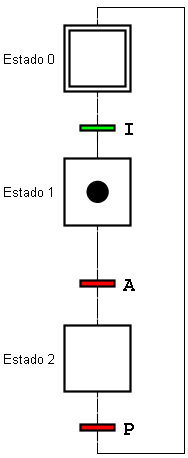
\includegraphics[scale=0.6]{figuras/grafcetSimples}
  \caption{Exemplo de um diagrama grafcet simples.}
  \label{fig:grafcetSimples}
\end{figure}

A evolução do sistema descrito em grafcet é dada pelo disparo das transições. Um transição dispara quando:
\begin{itemize}
  \item ela está ativa e
  \item todos os estados anteriores a ela estão ativos.
\end{itemize}

Quando uma transição dispara ela desativa todos os estados anteriores a ela (os estados acima) e ativa todos os posteriores (os abaixo). Por exemplo, se na figura \ref{fig:grafcetSimples} a condição A se tornasse verdadeira, como o único estado anterior, o Estado 1 está ativo, esta transição dispararia, desativando Estado 1 e ativando Estado 2. Esta sequência é mostrada na figura \ref{fig:grafcetDisparo}.
\begin{figure}[hbt]
  \centering
  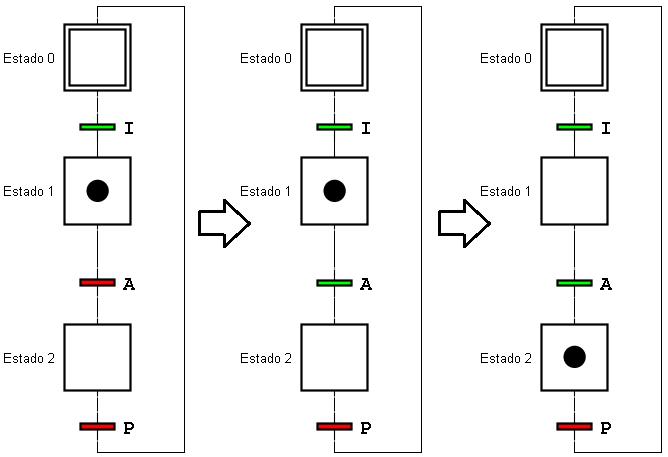
\includegraphics[scale=0.6]{figuras/grafcetDisparo}
  \caption{Sequência de disparo da transição A}
  \label{fig:grafcetDisparo}
\end{figure}

\section{Divergências e convergências}

No grafcet, pode-se ter um estado com mais de uma transição de saída, que pode levar para estados diferentes de acordo com qual transição dispare primeiro. A isto se chama uma \emph{divergência OU}, pois separa em dois caminhos excludentes. Da mesma forma, duas (ou mais) transições podem levar para o mesmo estado, o que se chama de convergência OU. A figura \ref{fig:grafcetdivOU} mostra um exemplo em que o sistema pode evoluir por dois caminhos diferentes, com o uso de divergência e convergência OU.

\begin{figure}[hbt]
  \centering
  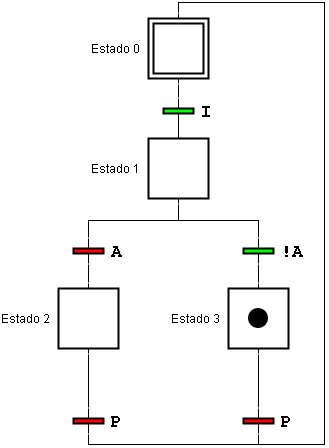
\includegraphics[scale=0.6]{figuras/grafcetdivOU}
  \caption{Exemplo de grafcet com divergência e convergência OU. O !A indica que a transição está ativa quando A for falso.}
  \label{fig:grafcetdivOU}
\end{figure}

Note-se na figura \ref{fig:grafcetdivOU} que o Estado 1 é obrigatoriamente transitório, pois ou A é verdadeiro e o sistema evolui imediatamente para o Estado 2 ou A é falso e o sistema ativa o Estado 3. É possível definir transições que estejam ativas ao mesmo tempo, neste caso o sistema evolui para a transição com maior prioridade -- ou a mais a esquerda ou se tiver uma prioridade explícita.

Diferente de uma máquina de estados, no grafcet é permitido que uma transição acione mais que um estado. Neste caso o sistema se divide em caminhos paralelos. Isto é chamado de divergência E e indicado por duas linhas horizontais, para diferenciar da divergência OU. Da mesma forma, uma convergência E liga vários estágios a uma única transição, transformando caminhos paralelos num único caminho. A figura \ref{fig:grafcetdivE} mostra um exemplo de divergência e convergência E.

\begin{figure}[hbt]
  \centering
  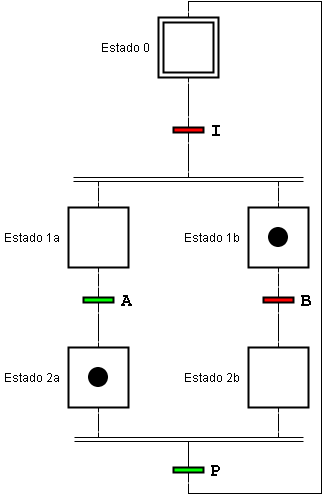
\includegraphics[scale=0.6]{figuras/grafcetdivE}
  \caption{Exemplo de grafcet com divergência e convergência E.}
  \label{fig:grafcetdivE}
\end{figure}

Note que, neste caso, mesmo com P ativo, o sistema não desativa o Estado 2a nem ativa Estado 0, pois como o Estado 2b não está ativo, a transição P não pode disparar.

\section{Ações}
Outra característica do grafcet é que podem ser definidas ações, ligadas a estados. O que exatamente compõem uma ação depende da implementação do grafcet. Peguemos dois exemplos: o JGrafchart e a SFC, que é a descrição de grafcet definida pela norma IEC61131.

No JGrafchart, uma ação pode ser uma definição de valor (um \emph{assignment}), da forma \lstinline|variavel = expressao|, uma chamada de subrotina (\emph{call}) ou uma variável booleana (\emph{bool}), que fica verdadeira enquanto o estado estiver ativo. Um qualificador de uma letra define o momento em que a ação é executada:
\begin{description}
  \item[S assignment|call;] Executa apenas uma vez, quando a etapa é ativada.
  \item[X assignment|call;] Executa apenas uma vez, quando a etapa é desativada.
  \item[P assignment|call;] Executa a cada ciclo enquanto a ação estiver acionada.
  \item[N bool;] Aciona a variável booleana enquanto a etapa estiver acionada.
  \item[A assignment|call;] Executa apenas uma vez, se a etapa for desativada por uma transição de exceção (apenas definida no JGrafchart).
\end{description}

Note-se que a ação \lstinline/N bool;/ é equivalente a \lstinline/P bool=1;/ e é presente para facilitar a escrita, já que tal operação é feita muitas vezes.

Toda etapa tem uma variável booleana x (\lstinline|<nome_da_etapa>.x|), que aciona quando a etapa é acionada, e uma variável de tempo em décimos de segundo t (\lstinline|<nome_da_etapa>.t|) e em segundos s (\lstinline|<nome_da_etapa>.s|).

As ações do SFC são do formato \textbf{\lstinline/qualificador funcao|variavel finalizado/}. \lstinline|finalizado| é uma variável opcional no caso de se usar uma função, que aciona quando a função termina, o que a torna útil para ser utilizada na transição de saída da etapa.

O qualificador pode ser qualquer um dos descritos na tabela \ref{tab:qualiSFC}. Pode-se não especificar o qualificador, onde o comportamento fica o mesmo de se usar o qualificador N. No caso da ação ser uma função, ele é executada sempre que ficar ativa. Todos os qualificadores que tem tempo acompanham um valor de tempo dado ou por uma variável ou por uma constante da forma \lstinline|T#4k|, onde k pode ser t (décimo de segundo), s (segundo), m, (minuto) ou h (hora).
\begin{table}[hbt]
  \caption{Qualificadores do SFC}
  \label{tab:qualiSFC}
  \centering

  \begin{tabularx}{\textwidth}{|c|X|}
  \hline

  \hline
  \textbf{Qualificador} & \textbf{descrição}\\
  \hline
   \textbf{N}  & Ativa a etapa estiver acionada. \\
   \textbf{S}  & Set -- ativa e mantém ativado mesmo depois de sair da etapa. \\
   \textbf{R}  & Reset -- desativa. \\
   \textbf{P}  & Ativa apenas no primeiro ciclo que a etapa estiver ativa. \\
   \textbf{L tempo}  & Ativa pelo tempo determinado enquanto a etapa estiver acionada.\\
   \textbf{SL tempo}  & Ativa pelo tempo determinado independente da etapa ainda estar acionada.\\
   \textbf{D tempo}  & Ativa após o tempo determinado enquanto a etapa estiver acionada.\\
   \textbf{SD tempo}  & Seta após o tempo determinado independente da etapa ainda estar acionada.\\
   \textbf{DS tempo}  & Seta após o tempo determinado se a etapa ainda estiver acionada.\\
  \hline

  \hline
  \end{tabularx}
\end{table}

\clearpage
\section{Níveis}
O Grafcet pode ser definido em 2 níveis de abstração: o 1 e o 2. O nível 1 serve como uma ferramenta de desenvolvimento, para analisar a partir do problema como um todo a sequência de etapas, as ações a serem realizadas em cada etapa e as condições de transição de uma etapa para outra. No nível 1 as ações e transições são descritas de forma ampla, para permitirem uma melhor visualização do processo pelo desenvolvedor. O resultado final é uma descrição dos requisitos daquelas etapas e transições e não serve como uma linguagem para programar um sistema.

Já o Grafcet nível 2 é propriamente uma linguagem de programação, com diferentes implementações. Uma delas é o SFC - \emph{Sequential Function Chart}, descrita no padrão IEC1131-3 para programação de CLPs. No SFC, cada ação corresponde a uma atuação nas saídas ou variáveis internas do CLP e cada transição corresponde a um valor binário obtido no CLP seja de entradas, seja de comparações de valores analógicos ou de tempo.

Desta forma o principal uso do grafcet é num projeto top-down, onde a partir do problema se desenvolve a sequência a ser seguida no grafcet nível 1, a partir deste se definem todas as entradas, saídas e condições necessárias para o controle automático daquela sequência e então programa-se o sistema usando grafcet nível 2.

Tomemos como exemplo uma tarefa relativamente simples: cozinhar um ovo. Considere-se o sistema da figura \ref{fig:cozinhar_ovo}, consistindo de uma panela, uma entrada de água, uma boca de fogão a gás e um mecanismo que solte o ovo na água.

\begin{figure}[!h]
\centering
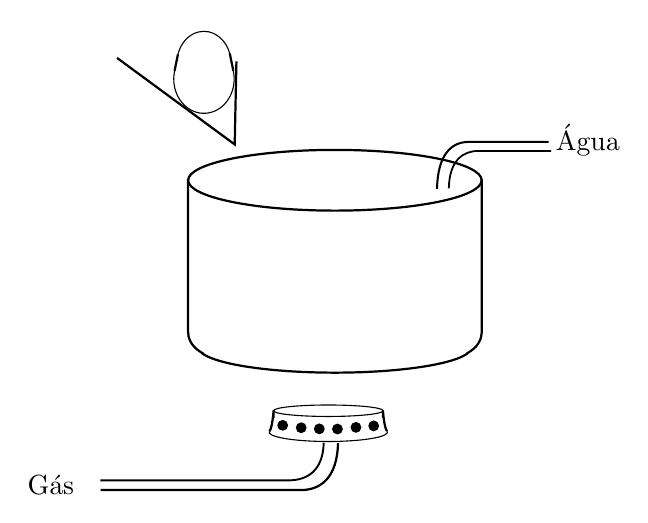
\begin{tikzpicture}[y=0.80pt, x=0.8pt,xscale=0.8,yscale=-0.8, inner sep=0pt, outer sep=0pt]
\begin{scope}[shift={(-99.03245,-288.02393)}]
    \path[draw=black,line join=miter,line cap=butt,line width=0.800pt]
      (354.2857,372.3622) .. controls (354.2857,381.8299) and (317.1893,389.5050) ..
      (271.4286,389.5050) .. controls (225.6678,389.5050) and (188.5714,381.8299) ..
      (188.5714,372.3622) .. controls (188.5714,362.8944) and (225.6678,355.2193) ..
      (271.4286,355.2193) .. controls (317.1893,355.2193) and (354.2857,362.8944) ..
      (354.2857,372.3622) -- cycle;
    \path[cm={{0.93174,0.0,0.0,0.83675,(18.52752,155.07504)}},draw=black,line
      join=miter,line cap=butt,line width=0.800pt] (351.5135,376.7594) .. controls
      (339.7757,385.9104) and (294.4050,391.3600) .. (250.1753,388.9315) .. controls
      (220.3437,387.2935) and (197.3850,382.3608) .. (190.5989,376.1313);
    \path[draw=black,line join=miter,line cap=butt,line width=0.800pt]
      (188.4845,371.6696) .. controls (188.4845,371.6696) and (188.4845,450.0421) ..
      (188.4845,457.6107) .. controls (188.4845,461.2730) and (190.0955,465.6973) ..
      (194.9956,468.8884) .. controls (198.4879,471.1627) and (197.0297,470.3066) ..
      (197.0297,470.3066);
    \path[draw=black,line join=miter,line cap=butt,line width=0.800pt]
      (354.3736,371.7266) .. controls (354.3736,371.7266) and (354.3736,450.0990) ..
      (354.3736,457.6677) .. controls (354.3736,461.3300) and (352.7625,465.7543) ..
      (347.8624,468.9454) .. controls (344.3701,471.2196) and (345.8283,470.3635) ..
      (345.8283,470.3635);
  \path[draw=black,line join=miter,line cap=butt,line width=0.800pt]
    (148.4437,303.3074) -- (214.8527,352.1376) -- (215.8294,305.2606);
  \begin{scope}[cm={{0.52126,0.0,0.0,0.55799,(132.31437,-4.68415)}}]
    \path[shift={(-3.38483,0)},draw=black] (160.1446,564.8529) .. controls
      (164.5668,583.4180) and (153.9497,602.2669) .. (136.4306,606.9532) .. controls
      (118.9114,611.6395) and (101.1244,600.3885) .. (96.7021,581.8235) .. controls
      (95.2554,575.7501) and (95.3885,569.3749) .. (97.0871,563.3753);
    \path[cm={{0.89621,0.0,0.0,-0.93321,(9.92999,1092.4228)}},draw=black]
      (160.3532,580.8939) .. controls (156.4154,599.5810) and (138.9277,611.3472) ..
      (121.2933,607.1743) .. controls (108.9462,604.2525) and (99.2953,594.0489) ..
      (96.5099,580.9713);
    \path[draw=black,line join=miter,line cap=butt,line width=0.800pt]
      (93.2329,565.0164) -- (96.8536,548.3611);
    \path[draw=black,line join=miter,line cap=butt,line width=0.800pt]
      (156.8450,565.0164) -- (153.0433,547.4560);
  \end{scope}
  \begin{scope}[shift={(0,10.0)}]
    \path[shift={(165.51847,-28.86265)},draw=black] (133.1216,521.3483) .. controls
      (133.1216,523.1376) and (119.2763,524.5880) .. (102.1973,524.5880) .. controls
      (85.1183,524.5880) and (71.2731,523.1376) .. (71.2731,521.3483) .. controls
      (71.2731,519.5591) and (85.1183,518.1086) .. (102.1973,518.1086) .. controls
      (119.2763,518.1086) and (133.1216,519.5591) .. (133.1216,521.3483) -- cycle;
    \path[cm={{0.95437,0.0,0.0,1.00307,(10.48141,-1.55578)}},draw=black]
      (304.2515,503.8934) .. controls (306.6885,506.7980) and (293.0976,509.4514) ..
      (273.8954,509.8200) .. controls (254.6932,510.1886) and (237.1512,508.1328) ..
      (234.7143,505.2283) .. controls (234.3214,504.7600) and (234.3437,504.2859) ..
      (234.7807,503.8186);
    \path[draw=black,line join=miter,line cap=butt,line width=0.800pt]
      (234.4953,503.9994) .. controls (236.1212,502.2258) and (236.7863,492.5444) ..
      (236.7863,492.5444) .. controls (236.7863,492.5444) and (236.7863,501.7823) ..
      (236.7863,492.2488);
    \path[draw=black,line join=miter,line cap=butt,line width=0.800pt]
      (300.8602,503.9994) .. controls (299.2343,502.2258) and (298.5692,492.5444) ..
      (298.5692,492.5444) .. controls (298.5692,492.5444) and (298.5692,501.7823) ..
      (298.5692,492.2488);
    \path[shift={(37.28111,-18.91723)},draw=black,fill=black] (248.7459,520.7984) ..
      controls (248.7459,522.2992) and (247.5293,523.5158) .. (246.0286,523.5158) ..
      controls (244.5278,523.5158) and (243.3112,522.2992) .. (243.3112,520.7984) ..
      controls (243.3112,519.2976) and (244.5278,518.0810) .. (246.0286,518.0810) ..
      controls (247.5293,518.0810) and (248.7459,519.2976) .. (248.7459,520.7984) --
      cycle;
    \path[shift={(26.8373,-17.9766)},draw=black,fill=black] (248.7459,520.7984) ..
      controls (248.7459,522.2992) and (247.5293,523.5158) .. (246.0286,523.5158) ..
      controls (244.5278,523.5158) and (243.3112,522.2992) .. (243.3112,520.7984) ..
      controls (243.3112,519.2976) and (244.5278,518.0810) .. (246.0286,518.0810) ..
      controls (247.5293,518.0810) and (248.7459,519.2976) .. (248.7459,520.7984) --
      cycle;
    \path[shift={(16.60251,-18.08111)},draw=black,fill=black] (248.7459,520.7984) ..
      controls (248.7459,522.2992) and (247.5293,523.5158) .. (246.0286,523.5158) ..
      controls (244.5278,523.5158) and (243.3112,522.2992) .. (243.3112,520.7984) ..
      controls (243.3112,519.2976) and (244.5278,518.0810) .. (246.0286,518.0810) ..
      controls (247.5293,518.0810) and (248.7459,519.2976) .. (248.7459,520.7984) --
      cycle;
    \path[shift={(6.36773,-18.7082)},draw=black,fill=black] (248.7459,520.7984) ..
      controls (248.7459,522.2992) and (247.5293,523.5158) .. (246.0286,523.5158) ..
      controls (244.5278,523.5158) and (243.3112,522.2992) .. (243.3112,520.7984) ..
      controls (243.3112,519.2976) and (244.5278,518.0810) .. (246.0286,518.0810) ..
      controls (247.5293,518.0810) and (248.7459,519.2976) .. (248.7459,520.7984) --
      cycle;
    \path[shift={(-4.07609,-20.0669)},draw=black,fill=black] (248.7459,520.7984) ..
      controls (248.7459,522.2992) and (247.5293,523.5158) .. (246.0286,523.5158) ..
      controls (244.5278,523.5158) and (243.3112,522.2992) .. (243.3112,520.7984) ..
      controls (243.3112,519.2976) and (244.5278,518.0810) .. (246.0286,518.0810) ..
      controls (247.5293,518.0810) and (248.7459,519.2976) .. (248.7459,520.7984) --
      cycle;
    \path[shift={(47.30687,-19.75335)},draw=black,fill=black] (248.7459,520.7984) ..
      controls (248.7459,522.2992) and (247.5293,523.5158) .. (246.0286,523.5158) ..
      controls (244.5278,523.5158) and (243.3112,522.2992) .. (243.3112,520.7984) ..
      controls (243.3112,519.2976) and (244.5278,518.0810) .. (246.0286,518.0810) ..
      controls (247.5293,518.0810) and (248.7459,519.2976) .. (248.7459,520.7984) --
      cycle;
  \end{scope}
  \path[draw=black,line join=miter,line cap=butt,line width=0.800pt]
    (273.1769,520.7233) .. controls (272.7485,540.4295) and (263.3238,547.2838) ..
    (252.1855,547.2838) .. controls (241.0472,547.2838) and (139.0890,547.2838) ..
    (139.0890,547.2838);
  \path[draw=black,line join=miter,line cap=butt,line width=0.692pt]
    (265.1049,520.6557) .. controls (264.7021,536.3302) and (255.8400,541.7823) ..
    (245.3666,541.7823) .. controls (234.8932,541.7823) and (139.0214,541.7823) ..
    (139.0214,541.7823);
  \path[fill=black] (97.967995,549.99866) node[above right] (text3077) {Gás};
  \path[draw=black,line join=miter,line cap=butt,line width=0.736pt]
    (329.0890,377.2838) .. controls (329.4517,357.5776) and (337.4309,350.7233) ..
    (346.8607,350.7233) .. controls (356.2906,350.7233) and (392.0864,350.7233) ..
    (392.0864,350.7233);
  \path[draw=black,line join=miter,line cap=butt,line width=0.638pt]
    (335.7362,376.9255) .. controls (336.0789,361.2509) and (343.6164,355.7989) ..
    (352.5243,355.7989) .. controls (361.4323,355.7989) and (393.4609,355.7989) ..
    (393.4609,355.7989);
  \path[fill=black] (396.19095,358.56888) node[above right] (text3085) {Água};
\end{scope}

\end{tikzpicture}
\caption{Sistema para cozinhar ovo sem sensores ou atuadores.}
\label{fig:cozinhar_ovo}
\end{figure}

Podemos inicialmente fazer um grafcet considerando que tudo dá sempre certo: ao iniciarmos o sistema, a panela enche de água, o ovo é colocado, o fogo acendido e aguarda-se até o ovo ficar pronto, de onde se retira a panela para tirar o ovo. Esta sequência é descrita pelo grafcet da figura \ref{fig:grafcetOvoOK}.

\begin{figure}[!h]
\centering
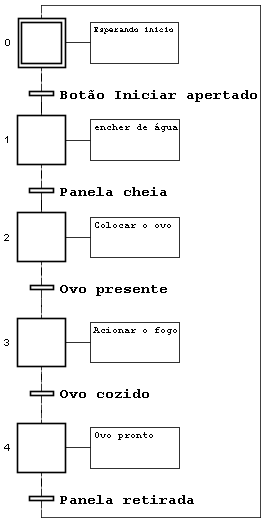
\includegraphics[scale=1]{figuras/ovoOK}
\caption{Diagrama grafcet nível 1 para cozinhar um ovo de forma otimista.}
\label{fig:grafcetOvoOK}
\end{figure}

Porém, problemas acontecem. Pode-se, por exemplo, esquecer de colocar a panela de volta antes de iniciar, faltar fogo ou acabar o ovo. Colocando todas estas condições a mais e defininindo o que fazer se elas acontecerem o grafcet cresce para o apresentado na figura \ref{fig:grafcetOvo1}.

\begin{figure}[!h]
\centering
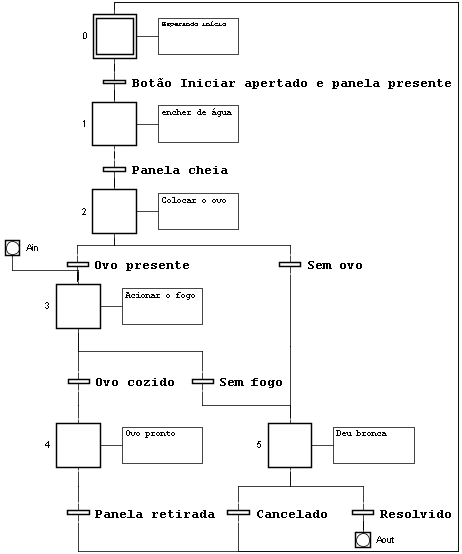
\includegraphics[scale=1]{figuras/ovoNivel1}

\caption{Diagrama grafcet nível 1 para cozinhar um ovo.}
\label{fig:grafcetOvo1}
\end{figure}

Com base neste diagrama, pode-se analisar agora quais são os sensores e atuadores necessários para esta tarefa, mostrados na figura \ref{fig:cozinhar_ovo2}. São eles:

\begin{description}
  \item[S\_PP] Sensor de presença para detectar a panela.
  \item[S\_N] Sensor de distância para obter o nível de água.
  \item[S\_G] Sensor de gás.
  \item[B\_I] Botão de início.
  \item[B\_OK] Botão de OK, para continuar se der bronca.
  \item[B\_C] Botão de cancelamento.
  \item[PO] Solenóide para abrir a portinhola do ovo.
  \item[VA] Válvula de controle da água.
  \item[VG] Válvula de controle do gás.
  \item[CENTELHA] para ligar o fogo.
  \item[ALARME] para indicar que deu errado.
\end{description}

\begin{figure}[!h]
\centering
\definecolor{c0000ff}{RGB}{0,0,255}
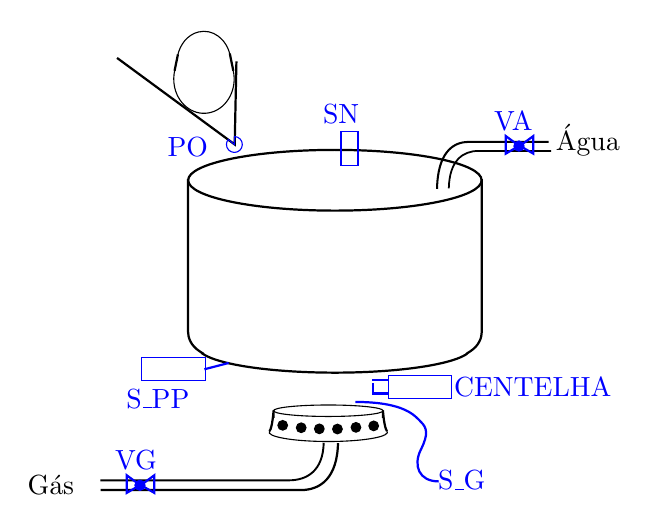
\begin{tikzpicture}[y=0.80pt, x=0.8pt,yscale=-0.8, xscale=0.8, inner sep=0pt, outer sep=0pt]
\begin{scope}[shift={(-99.03245,-288.02393)}]
    \path[draw=black,line join=miter,line cap=butt,line width=0.800pt]
      (354.2857,372.3622) .. controls (354.2857,381.8299) and (317.1893,389.5050) ..
      (271.4286,389.5050) .. controls (225.6678,389.5050) and (188.5714,381.8299) ..
      (188.5714,372.3622) .. controls (188.5714,362.8944) and (225.6678,355.2193) ..
      (271.4286,355.2193) .. controls (317.1893,355.2193) and (354.2857,362.8944) ..
      (354.2857,372.3622) -- cycle;
    \path[cm={{0.93174,0.0,0.0,0.83675,(18.52752,155.07504)}},draw=black,line
      join=miter,line cap=butt,line width=0.800pt] (351.5135,376.7594) .. controls
      (339.7757,385.9104) and (294.4050,391.3600) .. (250.1753,388.9315) .. controls
      (220.3437,387.2935) and (197.3850,382.3608) .. (190.5989,376.1313);
    \path[draw=black,line join=miter,line cap=butt,line width=0.800pt]
      (188.4845,371.6696) .. controls (188.4845,371.6696) and (188.4845,450.0421) ..
      (188.4845,457.6107) .. controls (188.4845,461.2730) and (190.0955,465.6973) ..
      (194.9956,468.8884) .. controls (198.4879,471.1627) and (197.0297,470.3066) ..
      (197.0297,470.3066);
    \path[draw=black,line join=miter,line cap=butt,line width=0.800pt]
      (354.3736,371.7266) .. controls (354.3736,371.7266) and (354.3736,450.0990) ..
      (354.3736,457.6677) .. controls (354.3736,461.3300) and (352.7625,465.7543) ..
      (347.8624,468.9454) .. controls (344.3701,471.2196) and (345.8283,470.3635) ..
      (345.8283,470.3635);
  \path[draw=black,line join=miter,line cap=butt,line width=0.800pt]
    (148.4437,303.3074) -- (214.8527,352.1376) -- (215.8294,305.2606);
  \begin{scope}[cm={{0.52126,0.0,0.0,0.55799,(132.31437,-4.68415)}}]
    \path[shift={(-3.38483,0)},draw=black] (160.1446,564.8529) .. controls
      (164.5668,583.4180) and (153.9497,602.2669) .. (136.4306,606.9532) .. controls
      (118.9114,611.6395) and (101.1244,600.3885) .. (96.7021,581.8235) .. controls
      (95.2554,575.7501) and (95.3885,569.3749) .. (97.0871,563.3753);
    \path[cm={{0.89621,0.0,0.0,-0.93321,(9.92999,1092.4228)}},draw=black]
      (160.3532,580.8939) .. controls (156.4154,599.5810) and (138.9277,611.3472) ..
      (121.2933,607.1743) .. controls (108.9462,604.2525) and (99.2953,594.0489) ..
      (96.5099,580.9713);
    \path[draw=black,line join=miter,line cap=butt,line width=0.800pt]
      (93.2329,565.0164) -- (96.8536,548.3611);
    \path[draw=black,line join=miter,line cap=butt,line width=0.800pt]
      (156.8450,565.0164) -- (153.0433,547.4560);
  \end{scope}
  \begin{scope}[shift={(0,10.0)}]
    \path[shift={(165.51847,-28.86265)},draw=black] (133.1216,521.3483) .. controls
      (133.1216,523.1376) and (119.2763,524.5880) .. (102.1973,524.5880) .. controls
      (85.1183,524.5880) and (71.2731,523.1376) .. (71.2731,521.3483) .. controls
      (71.2731,519.5591) and (85.1183,518.1086) .. (102.1973,518.1086) .. controls
      (119.2763,518.1086) and (133.1216,519.5591) .. (133.1216,521.3483) -- cycle;
    \path[cm={{0.95437,0.0,0.0,1.00307,(10.48141,-1.55578)}},draw=black]
      (304.2515,503.8934) .. controls (306.6885,506.7980) and (293.0976,509.4514) ..
      (273.8954,509.8200) .. controls (254.6932,510.1886) and (237.1512,508.1328) ..
      (234.7143,505.2283) .. controls (234.3214,504.7600) and (234.3437,504.2859) ..
      (234.7807,503.8186);
    \path[draw=black,line join=miter,line cap=butt,line width=0.800pt]
      (234.4953,503.9994) .. controls (236.1212,502.2258) and (236.7863,492.5444) ..
      (236.7863,492.5444) .. controls (236.7863,492.5444) and (236.7863,501.7823) ..
      (236.7863,492.2488);
    \path[draw=black,line join=miter,line cap=butt,line width=0.800pt]
      (300.8602,503.9994) .. controls (299.2343,502.2258) and (298.5692,492.5444) ..
      (298.5692,492.5444) .. controls (298.5692,492.5444) and (298.5692,501.7823) ..
      (298.5692,492.2488);
    \path[shift={(37.28111,-18.91723)},draw=black,fill=black] (248.7459,520.7984) ..
      controls (248.7459,522.2992) and (247.5293,523.5158) .. (246.0286,523.5158) ..
      controls (244.5278,523.5158) and (243.3112,522.2992) .. (243.3112,520.7984) ..
      controls (243.3112,519.2976) and (244.5278,518.0810) .. (246.0286,518.0810) ..
      controls (247.5293,518.0810) and (248.7459,519.2976) .. (248.7459,520.7984) --
      cycle;
    \path[shift={(26.8373,-17.9766)},draw=black,fill=black] (248.7459,520.7984) ..
      controls (248.7459,522.2992) and (247.5293,523.5158) .. (246.0286,523.5158) ..
      controls (244.5278,523.5158) and (243.3112,522.2992) .. (243.3112,520.7984) ..
      controls (243.3112,519.2976) and (244.5278,518.0810) .. (246.0286,518.0810) ..
      controls (247.5293,518.0810) and (248.7459,519.2976) .. (248.7459,520.7984) --
      cycle;
    \path[shift={(16.60251,-18.08111)},draw=black,fill=black] (248.7459,520.7984) ..
      controls (248.7459,522.2992) and (247.5293,523.5158) .. (246.0286,523.5158) ..
      controls (244.5278,523.5158) and (243.3112,522.2992) .. (243.3112,520.7984) ..
      controls (243.3112,519.2976) and (244.5278,518.0810) .. (246.0286,518.0810) ..
      controls (247.5293,518.0810) and (248.7459,519.2976) .. (248.7459,520.7984) --
      cycle;
    \path[shift={(6.36773,-18.7082)},draw=black,fill=black] (248.7459,520.7984) ..
      controls (248.7459,522.2992) and (247.5293,523.5158) .. (246.0286,523.5158) ..
      controls (244.5278,523.5158) and (243.3112,522.2992) .. (243.3112,520.7984) ..
      controls (243.3112,519.2976) and (244.5278,518.0810) .. (246.0286,518.0810) ..
      controls (247.5293,518.0810) and (248.7459,519.2976) .. (248.7459,520.7984) --
      cycle;
    \path[shift={(-4.07609,-20.0669)},draw=black,fill=black] (248.7459,520.7984) ..
      controls (248.7459,522.2992) and (247.5293,523.5158) .. (246.0286,523.5158) ..
      controls (244.5278,523.5158) and (243.3112,522.2992) .. (243.3112,520.7984) ..
      controls (243.3112,519.2976) and (244.5278,518.0810) .. (246.0286,518.0810) ..
      controls (247.5293,518.0810) and (248.7459,519.2976) .. (248.7459,520.7984) --
      cycle;
    \path[shift={(47.30687,-19.75335)},draw=black,fill=black] (248.7459,520.7984) ..
      controls (248.7459,522.2992) and (247.5293,523.5158) .. (246.0286,523.5158) ..
      controls (244.5278,523.5158) and (243.3112,522.2992) .. (243.3112,520.7984) ..
      controls (243.3112,519.2976) and (244.5278,518.0810) .. (246.0286,518.0810) ..
      controls (247.5293,518.0810) and (248.7459,519.2976) .. (248.7459,520.7984) --
      cycle;
  \end{scope}
  \path[draw=black,line join=miter,line cap=butt,line width=0.800pt]
    (273.1769,520.7233) .. controls (272.7485,540.4295) and (263.3238,547.2838) ..
    (252.1855,547.2838) .. controls (241.0472,547.2838) and (139.0890,547.2838) ..
    (139.0890,547.2838);
  \path[draw=black,line join=miter,line cap=butt,line width=0.692pt]
    (265.1049,520.6557) .. controls (264.7021,536.3302) and (255.8400,541.7823) ..
    (245.3666,541.7823) .. controls (234.8932,541.7823) and (139.0214,541.7823) ..
    (139.0214,541.7823);
  \path[fill=black] (97.967995,549.99866) node[above right] (text3077) {Gás};
  \path[draw=black,line join=miter,line cap=butt,line width=0.736pt]
    (329.0890,377.2838) .. controls (329.4517,357.5776) and (337.4309,350.7233) ..
    (346.8607,350.7233) .. controls (356.2906,350.7233) and (392.0864,350.7233) ..
    (392.0864,350.7233);
  \path[draw=black,line join=miter,line cap=butt,line width=0.638pt]
    (335.7362,376.9255) .. controls (336.0789,361.2509) and (343.6164,355.7989) ..
    (352.5243,355.7989) .. controls (361.4323,355.7989) and (393.4609,355.7989) ..
    (393.4609,355.7989);
  \path[fill=black] (396.19095,358.56888) node[above right] (text3085) {Água};
  \path[draw=c0000ff,rounded corners=0.0000cm] (274.8555,344.6107) rectangle
    (284.4550,363.8097);
  \path[text=c0000ff] (264.7507,340.06354) node[above right] (text3091) {SN};
  \path[shift={(103.79863,289.84629)},draw=c0000ff] (111.0562,57.8371) .. controls
    (113.5319,57.9323) and (115.4616,60.0164) .. (115.3663,62.4920) .. controls
    (115.2711,64.9676) and (113.1870,66.8973) .. (110.7114,66.8021) .. controls
    (108.2358,66.7069) and (106.3061,64.6228) .. (106.4013,62.1472) .. controls
    (106.4392,61.1629) and (106.8000,60.2184) .. (107.4280,59.4596) --
    (110.8838,62.3196) -- cycle;
  \path[text=c0000ff] (176.97354,359.03479) node[above right] (text3097) {PO};
  \path[shift={(99.03245,288.02393)},draw=c0000ff,rounded corners=0.0000cm]
    (63.3622,184.2778) rectangle (99.2487,197.1745);
  \path[shift={(99.03245,288.02393)},draw=c0000ff,line join=miter,line
    cap=butt,line width=0.800pt] (98.7270,191.0482) .. controls
    (112.6043,187.4797) and (112.4061,187.4797) .. (112.4061,187.4797);
  \path[text=c0000ff] (153.71358,501.07755) node[above right] (text3105) {S\_PP};
  \begin{scope}[shift={(-4.37896,11.89482)}]
    \path[shift={(109.53954,277.51684)},draw=c0000ff,fill=c0000ff]
      (59.0776,255.1811) .. controls (59.0776,256.7687) and (57.7906,258.0557) ..
      (56.2030,258.0557) .. controls (54.6154,258.0557) and (53.3285,256.7687) ..
      (53.3285,255.1811) .. controls (53.3285,253.5935) and (54.6154,252.3065) ..
      (56.2030,252.3065) .. controls (57.7906,252.3065) and (59.0776,253.5935) ..
      (59.0776,255.1811) -- cycle;
    \path[shift={(99.03245,288.02393)},draw=c0000ff,line join=miter,line
      cap=butt,line width=0.800pt] (66.8093,244.5749) -- (59.2477,248.9406) --
      (59.2477,239.0240) -- cycle;
    \path[draw=c0000ff,line join=miter,line cap=butt,line width=0.800pt]
      (166.2801,532.5988) -- (173.8417,536.9645) -- (173.8417,527.0479) -- cycle;
  \end{scope}
  \path[text=c0000ff] (147.31708,535.6076) node[above right] (text3122) {VG};
  \begin{scope}[shift={(209.61758,-179.63899)}]
    \path[shift={(109.53954,277.51684)},draw=c0000ff,fill=c0000ff]
      (59.0776,255.1811) .. controls (59.0776,256.7687) and (57.7906,258.0557) ..
      (56.2030,258.0557) .. controls (54.6154,258.0557) and (53.3285,256.7687) ..
      (53.3285,255.1811) .. controls (53.3285,253.5935) and (54.6154,252.3065) ..
      (56.2030,252.3065) .. controls (57.7906,252.3065) and (59.0776,253.5935) ..
      (59.0776,255.1811) -- cycle;
    \path[shift={(99.03245,288.02393)},draw=c0000ff,line join=miter,line
      cap=butt,line width=0.800pt] (66.8093,244.5749) -- (59.2477,248.9406) --
      (59.2477,239.0240) -- cycle;
    \path[draw=c0000ff,line join=miter,line cap=butt,line width=0.800pt]
      (166.2801,532.5988) -- (173.8417,536.9645) -- (173.8417,527.0479) -- cycle;
  \end{scope}
  \path[text=c0000ff] (361.31363,344.07382) node[above right] (text3122-9) {VA};
  \path[draw=c0000ff,line join=miter,line cap=butt,line width=0.800pt]
    (282.9510,497.5344) .. controls (310.9874,497.5344) and (316.5946,505.3846) ..
    (319.9590,508.7490) .. controls (323.3234,512.1133) and (324.4448,515.4777) ..
    (319.9590,524.4493) .. controls (315.4732,533.4210) and (318.8376,542.3926) ..
    (330.0521,542.3926);
  \path[text=c0000ff] (329.78195,547.05719) node[above right] (text3161) {S\_G};
  \path[draw=c0000ff,rounded corners=0.0000cm] (301.4550,482.6751) rectangle
    (337.3415,495.5719);
  \path[text=c0000ff] (338.7536,494.34882) node[above right] (text3183) {CENTELHA};
  \path[shift={(99.03245,288.02393)},draw=c0000ff,line join=miter,line
    cap=butt,line width=0.800pt] (202.5627,204.7443) -- (193.7313,204.7443) --
    (193.7313,198.9969);
  \path[shift={(99.03245,288.02393)},draw=c0000ff,line join=miter,line
    cap=butt,line width=0.800pt] (202.2824,197.1745) -- (193.5911,197.1745);
\end{scope}
\end{tikzpicture}
\caption{Sistema para cozinhar ovo com sensores e atuadores.}
\label{fig:cozinhar_ovo2}
\end{figure}

Então com base nos sensores e atuadores presentes, podemos fazer o grafcet nível 2 (figura \ref{fig:grafcetOvo2}, descrevendo as ações e transições de acordo com estas entradas e saídas.

\begin{figure}[!h]
\centering
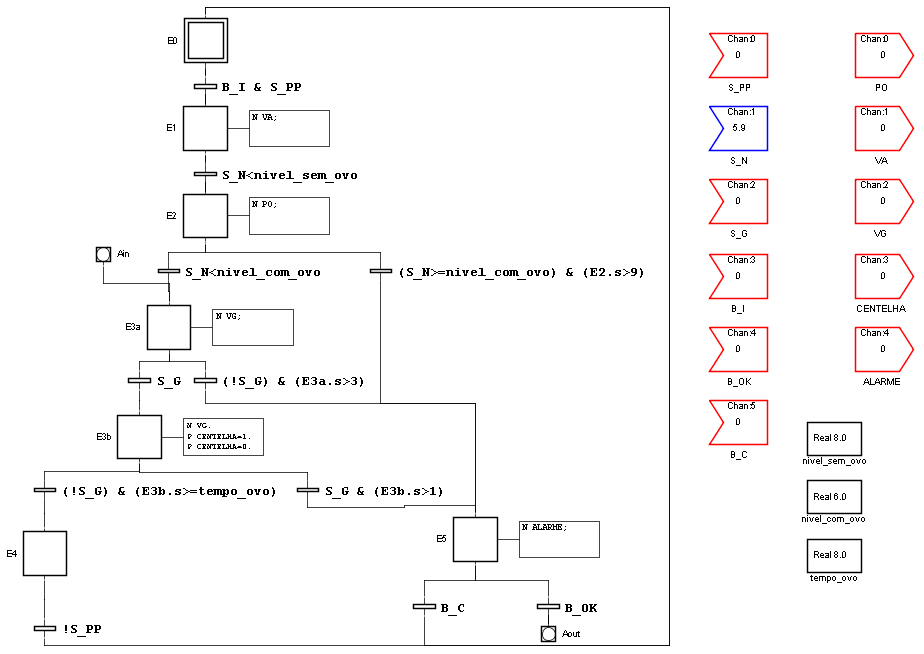
\includegraphics[width=\textwidth]{figuras/ovoNivel2}
\caption{Diagrama grafcet nível 2 para cozinhar um ovo.}
\label{fig:grafcetOvo2}
\end{figure}

